\chapter{Objetivos}
\label{ch:objetivos}

%* Listo
Bajo la premisa de realizar un \textbf{analizador USB \emph{hardware} de bajo coste} con herramientas y utilidades de código libre, el presente Trabajo Fin de Grado se ha descompuesto en varios objetivos parciales, estos siguen siempre una metodología SMART, es decir, deben ser Simples, Medibles, Acordados, Realista y Temporizados.

%* Listo
\section{Selección de componentes \emph{hardware}}
Debido a la flexibilidad que supone utilizar una FPGA\cite{monmasson2007fpga}, se propone diseñar el sistema de captura a partir de una. Por otra parte, ya que existen circuitos especializados en procesar capas física USB, es de gran interés incluir uno de ellos\footnote{La idea de utilizar un integrado especializado, se obtiene del sistema \emph{USB Sniffer} planteado por \emph{Ultra-Embedded}, nombrado en el capitulo~\ref{ch:antecedentes} de antecedentes.}, pudiendo abstraer de esa forma ciertas partes de la comunicación USB de poco interés, y reduciendo en cierta medidas posibles errores de sincronización.

Se deben buscar por tanto, todos aquellos componentes necesarios, de la forma más económica posible, para elaborar el sistema de captura. Seguidamente, se ha de elegir como se conexionan mutuamente.

%* Listo
\section{Implementación de memoria \emph{FIFO}}
Diseño e implementación de un módulo en lenguaje Verilog que actúe como memoria \emph{FIFO}. Este será capaz de almacenar información de tal manera que el primer $bit$ introducido sea el primero en ser recuperado.

Dado que la FPGA a utilizar dispone de varios bloques de RAM específicos, se utilizarán varios de estos para no depender unicamente de registros, consiguiendo una mayor capacidad de almacenamiento, con un circuito lo mayor optimizado posible.

La gran mayoría los módulos a diseñar dependen en gran medida de este tipo de memoria, por lo que es esencial disponer de ella en el la mayor brevedad posible, a su vez, y debido a su gran utilidad, la velocidad\cite{rose1993architecture} máxima a la que puede funcionar el sistema en su conjunto está dada por su velocidad de escritura/lectura de datos.

En la figura~\ref{fig:FIFO_info} se muestra un esquema del resultado esperado.

\begin{figure}[htb]
    \centering
    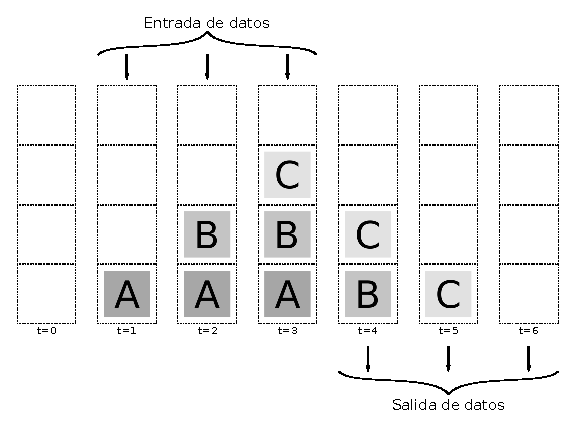
\includegraphics[width=80mm]{esquemas/FIFO_bw.eps}
    \caption{Esquema de funcionamiento de una memoria \emph{FIFO}.}
    \label{fig:FIFO_info}
\end{figure}



%* Listo
\section{Implementación de un sistema de comunicación serie}
Diseño e implementación de un sistema en lenguaje Verilog que sea capaz de comunicarse bidireccionalmente usando un puerto serie simple\cite{design-uart-vhdl}, pudiendo conectarse a él por medio del circuito integrado FTDI FT2232HL\footnote{Circuito encargado de convertir una conexión \emph{USB High Speed} a dos protocolos configurables distintos. En el caso de la placa de desarrollo \emph{IceStick}, se utiliza un canal para programar la memoria \emph{Flash} SPI utilizada por la FPGA, y otro para proporcionar una comunicación UART hacia el equipo.} (disponible en la placa de desarrollo \emph{IceStick}\cite{icestickmanual}), o utilizando un equipo externo compatible.

Por dicho puerto, la FPGA transmitirá tanto la trama USB capturada como información del bus, y recibirá los comandos que debe seguir.

En la figura~\ref{fig:serie_esquema} se muestra una señal típica serie, esta es la señal que debe ser capturada y generada en la FPGA.

\begin{figure}[htb]
    \centering
    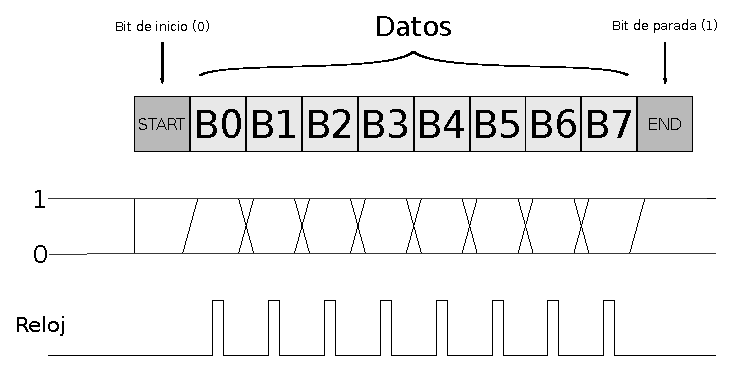
\includegraphics[height=52mm]{esquemas/serie.eps}
    \caption{Señal típica de una comunicación serie.}
    \label{fig:serie_esquema}
\end{figure}

A su vez, este objetivo se puede descomponer en varios subobjetivos.

%* Listo
\subsection{Diseño de un módulo de emisión serie}
Módulo capaz de controlar los datos almacenados en una memoria \emph{FIFO}, para posteriormente transmitirlos por el puerto serie.

%* Listo
\subsection{Diseño de un módulo de recepción serie}
Módulo capaz almacenar en una memoria \emph{FIFO} los datos paralelizados capturados en el puerto serie.



%* Listo
\section{Implementación de un sistema que procese el protocolo ULPI}
Diseño e implementación de un sistema en lenguaje Verilog capaz de comunicarse con otros dispositivos compatibles con el protocolo ULPI (\emph{UTMI+ Low Pin Interface}), siendo en este caso, el integrado USB3300 de \emph{Microchip}, encargado de la capa física USB.

Todas las características y casos del protocolo ULPI están completamente definidas tanto en la hoja de especificaciones del propio protocolo\cite{ulpi-specs} como en la hoja de características del circuito integrado USB3300\cite{microchip:usb3300}. Hay que destacar que el bus consta de una señal de reloj a $60MHz$ a la que se referencia el resto de señales (\emph{CLK}), 8 señales de datos bidireccionales paralelos (\emph{DATA}), una señal de control de dirección (\emph{DIR}) y dos señales extra de control (\emph{STP} y \emph{NXT}).

Puesto que unicamente queremos obtener de forma pasiva los datos USB, de los cuatro posibles modos de funcionamiento ULPI, escritura de registros, lectura de registros, recepción de datos USB y envío de datos USB, solo es interesante diseñar los tres primeros, por lo que este objetivo se puede dividir en las siguientes partes.

%* Listo
\subsection{Diseño de un módulo de escritura de registros ULPI}
Módulo capaz de generar y procesar las señales ULPI necesarias para almacenar un valor arbitrario de $8~bits$, en un registro del integrado conectado por ULPI.

En la figura~\ref{fig:ULPI_REG_WRITE} se puede apreciar la comunicación básica usada para realizar dicha escritura.
\begin{figure}[hbt]
    \centering
    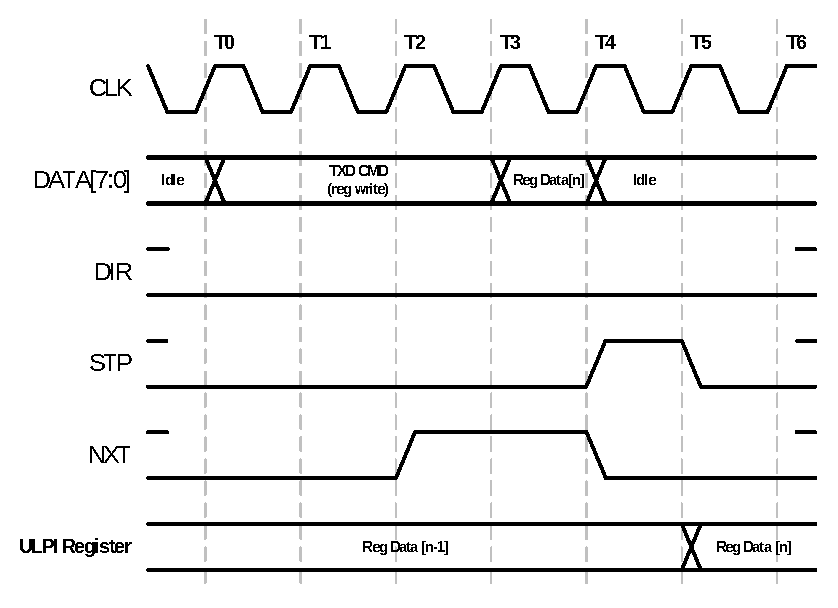
\includegraphics[width=90mm]{datasheets/USB3300_REG_WRITE.eps}
    \caption{Trama de escritura de registros ULPI.}
    \label{fig:ULPI_REG_WRITE}
\end{figure}

%* Listo
\subsection{Diseño de un módulo de lectura de registros ULPI}
Módulo capaz de generar y procesar las señales ULPI necesarias para obtener un valor almacenado en un registro arbitrario del integrado conectado por ULPI.

En la figura~\ref{fig:ULPI_REG_READ} se puede apreciar la comunicación básica usada para realizar dicha lectura.
\begin{figure}[hbt]
    \centering
    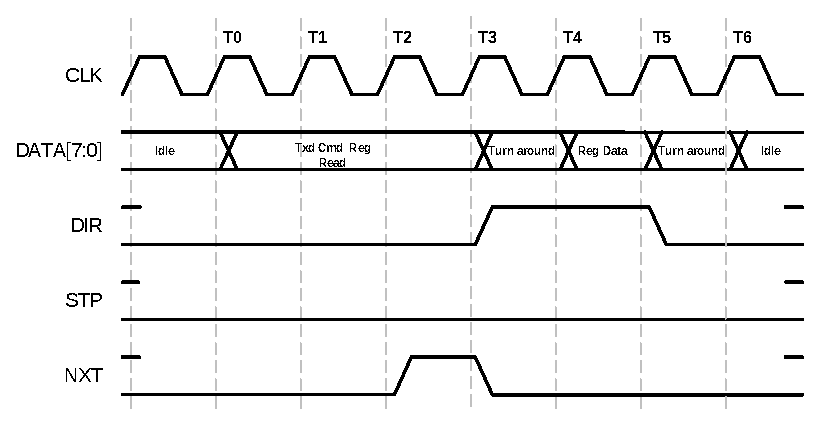
\includegraphics[width=90mm]{datasheets/USB3300_REG_READ.eps}
    \caption{Trama de lectura de registros ULPI.}
    \label{fig:ULPI_REG_READ}
\end{figure}

%* Listo
\subsection{Diseño de un módulo de captación USB}
Módulo que ante la llegada de datos USB, sea capaz de procesar las señales ULPI para obtener y clasificar la trama transmitida. En la figura~\ref{fig:ULPI_RECV} se puede apreciar la comunicación básica existente durante la lectura de datos.
\begin{figure}[hbt]
    \centering
    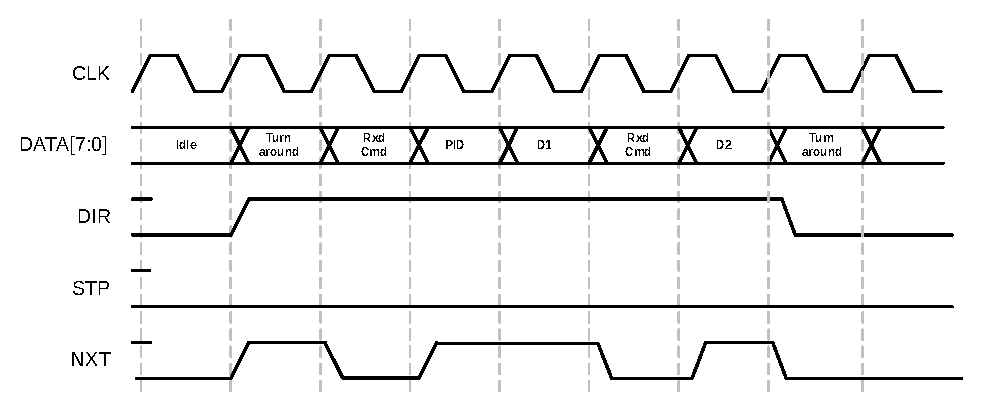
\includegraphics[width=90mm]{datasheets/USB3300_RECV.eps}
    \caption{Trama ULPI de recepción de datos USB.}
    \label{fig:ULPI_RECV}
\end{figure}



%* Listo
\section{Implementación de un sistema que gestione el envío de datos}
Diseño e implementación de un módulo en lenguaje Verilog, que gestione el envío al PC de los datos capturados. Además, sería interesante añadir una memoria intermedia en la que almacenar los datos antes de su envío, aminorando posibles perdidas.



%* Listo
\section{Implementación de un sistema que gestione los comandos entrantes}
Diseño e implementación de un módulo en lenguaje Verilog, que ante cualquier petición realizada por el usuario por el puerto serie anterior, deberá ser capaz de procesarla, obteniendo sus diversas partes (por ejemplo, dirección y datos en una petición de escritura de registro) y las almacenará temporalmente hasta que se puedan ejecutar.



% %* Listo
% \section{Implementación de un sistema que gestione todos los módulos}
% Una vez todos los módulos anteriores estén finalizados, es necesaria una sincronización entre todos ellos que permita obtener el resultado deseado. Por ello, se diseñará un módulo que envíe las señales de control pertinentes al resto de módulos dependiendo de las diversas entradas o registros internos de control.



%* Listo
\section{Creación de una aplicación de control}
Tras la finalización de la parte \emph{hardware}, es necesaria una aplicación, que conectándose por medio del puerto serie anteriormente implementado, sea capaz de en primer lugar enviar los diversos comandos necesarios para el correcto funcionamiento del sistema, y en segundo lugar, reciba los datos capturados de interés.

Debe ser como mínimo capaz de realizar las siguientes tareas.
\begin{itemize}
    \item Proveer de una sencilla interfaz en la que controlar todos los aspectos del sistema de captura.
    \item Controlar y procesar los datos entrantes y salientes del puerto serie.
    \item Almacenar los datos capturados en un archivo que permita un fácil análisis futuro, preferiblemente \emph{PCAP}\cite{tcpdump:pcap}.
\end{itemize}



% \section{Limitaciones en su ...}
% A la hora de desarrollar todos los objetivos anteriores, hay que tener presente todas aquellas limitaciones, principalmente los impuestos por la FPGA.

% \begin{itemize}
%     \item Existencia de unicamente 16 bloques de RAM de $4Kbits$ cada uno.
%     \item 
% \end{itemize}


% \chapter{Objetivos}
% \label{ch:objetivos-plantilla}

% Primero enumera los objetivos, no los resumas ni los redactes en un párrafo.  Cada uno de los objetivos de un proyecto debe ser SMART:

% \begin{description}
% \item[Simple] Cada objetivo tiene que ser independiente, tener sentido por sí mismo y más o menos indivisible.  Si no es suficientemente indivisible, pero tiene sentido como una entidad independiente, debes descomponerlo en subobjetivos.
% \item[Medible] Tiene que ser posible medir el grado de consecución al final del TFG.
% \item[Acordado] Los objetivos no los pones tú solo.  Deben partir de un acuerdo con tu director.
% \item[Realista] No pongas objetivos muy ambiciosos. Basta con que resuelva el problema de la forma más simple posible.  Si superas los objetivos nadie se va a quejar.  El director se encargará de que tampoco sean demasiado poco ambiciosos.
% \item[Temporizado] Un objetivo debe tener un marco temporal. Si no es así el objetivo podría no cumplirse nunca.  Es difícil poner límites temporales muy estrictos en un primer proyecto de ingeniería, pero al menos acota.
% \end{description}

% Tras cada objetivo puedes añadir párrafos ampliando la descripción del objetivo, describiendo los límites y justificándolos.  También puedes describir de qué se parte.  Si es posible debería quedar plenamente justificado que se trata de objetivos SMART.  Considera tanto límites intrínsecos (inherentes a la definición del proyecto) como extrínsecos (limitaciones presupuestarias, equipamiento disponible, etc).